\chapter{Introduction}

\label{ch:intro}

The Mu2e Raw Data Mover (RDM) System is an element of Mu2e Data Processing
and Computing (DPC)~\cite{DPC}, an L2 project within Mu2e Experiment Operations Plan~\cite{PEOP}.
Its purpose is to move data
that is produced by the online system to long term storage;
for most data, the long term storage will be files on tape
but, for some data, it will be in one of the offline databases.
Some data may also reside transiently in disk files so that
it is readily avaialble for the follow-on data processing steps.

Other functions of the RDM include:
\begin{enumerate}
\item Updating the file catalog to include meta-data and file location(s).
\item Any splitting/joining or other reshaping of files that is needed to match the needs of downstream processing.
\item Managing the free space in the online disk buffer
\item Copy/mirror subsets of the online databases to the offline databases
\item Move miscellaneous other data, such as the output of the online Data Quality Monitoring (DQM) system, to long term storage.
\end{enumerate}

The current plan is that the offline data processing workflows will be driven by updates to the file catalog;
so the RDM does not need other hooks into those workflows.

%The operation and maintenance of the Mu2e building router and the network between the Mu2e Hall and the computer center
%is the responsibility of the Fermilab Core Computing Division (CCD).
%The DPS has the responsibility to be the interface between Mu2e and CCD regarding this network.
%Details of this responsbility are in Section~\fixme{reference the appropriate section}.


The main body of this document will describe a view of the
Mu2e Trigger and Data Acquisition system (TDAQ) as seen from the RDM perspective.
The cartoon picture is that TDAQ writes files to a disk buffer and RDM drains the disk buffer.
However, there are about 20 logical data streams, some tightly coupled to each
other, some loosely coupled to the others and others independent of the others.
Understanding the relationships among the data streams and their implications
for downstream processing are the starting point for designing the RDM.

This document includes additional information that is not written down concisely
in other places and is needed either to frame the description of the data streams
or to inform requirements.


The RDM owns no hardware.  It uses hardware that is owned and maintained
by the Mu2e TDAQ group,
by the Fermilab Scientific Computing Division (SCD)
and by the Fermilab Core Computing Division (CCD).
The only M\&S items within RDM are to pay CCD for router maintenance,
and its end-of-service-life replacement, as described in Appendix~\ref{app:RouterAndNetwork}.

In early planning for the Mu2e DPC, what is now called the RDM was called the Data Logging System.
However that name is too close to two related concepts in the online world:
the {\code artdaq::DataLogger} processes that run on the Data Logger nodes at the end of the TDAQ
processing chain.  The name was changed to RDM to avoid confusion with these other uses of Data Logger.

\section{Conventions Used in this Document}

In this document the word ``computer center'' is used as a collective noun for the
Feynman Computing Center (FCC) and the Grid Computing Center (GCC).
When it is important to distinguish the two, one of the two will be named explicitly.
This choice also allows future changes to the computing center infrastructure over the
lifetime of Mu2e.

The DPC is not part of the Mu2e Construction Project but it is part of Mu2e Operations
and pre-Operations.
In various places, this document refers to ``Mu2e groups'', such as the TDAQ group.
Sometimes this will mean an L2 group within the Mu2e Construction Project and at other
times it will mean a group within the Mu2e Operations or Pre-Operations organization.
Most of the time it will not be important to distinguish between these different meanings
of group; when it is important, it will be stated explicitly.


\chapter{Background Information}
\label{chap:BackgroundInfo}
This Chapter describes the view of the TDAQ and the computer center as seen by the RDM.

\section{Block Diagram}
\label{sec:BlockDiagram}

Figure~\ref{fig:blockdiagram} shows a block diagram of the major elements involved
in the data flow from the experiment hardware to long term storage.
All elements in the left hand dot-dashed box are located in the Mu2e Hall
and, except for the Mu2e building router, are the responsbility of the various Mu2e groups.
All elements in the right hand dot-dashed box are located in the computer center
and are the responsibility of SCD; the internal details of the SCD-managed resources
are not shown and the RDM will treat these resources as a interconnected, coherent whole.
The Mu2e building router and the optical fibre that connects that router
to the computer center are the responsibility of CCD;
see Appendix~\ref{app:RouterAndNetwork} for details.

\begin{figure}[tbp]
\centering
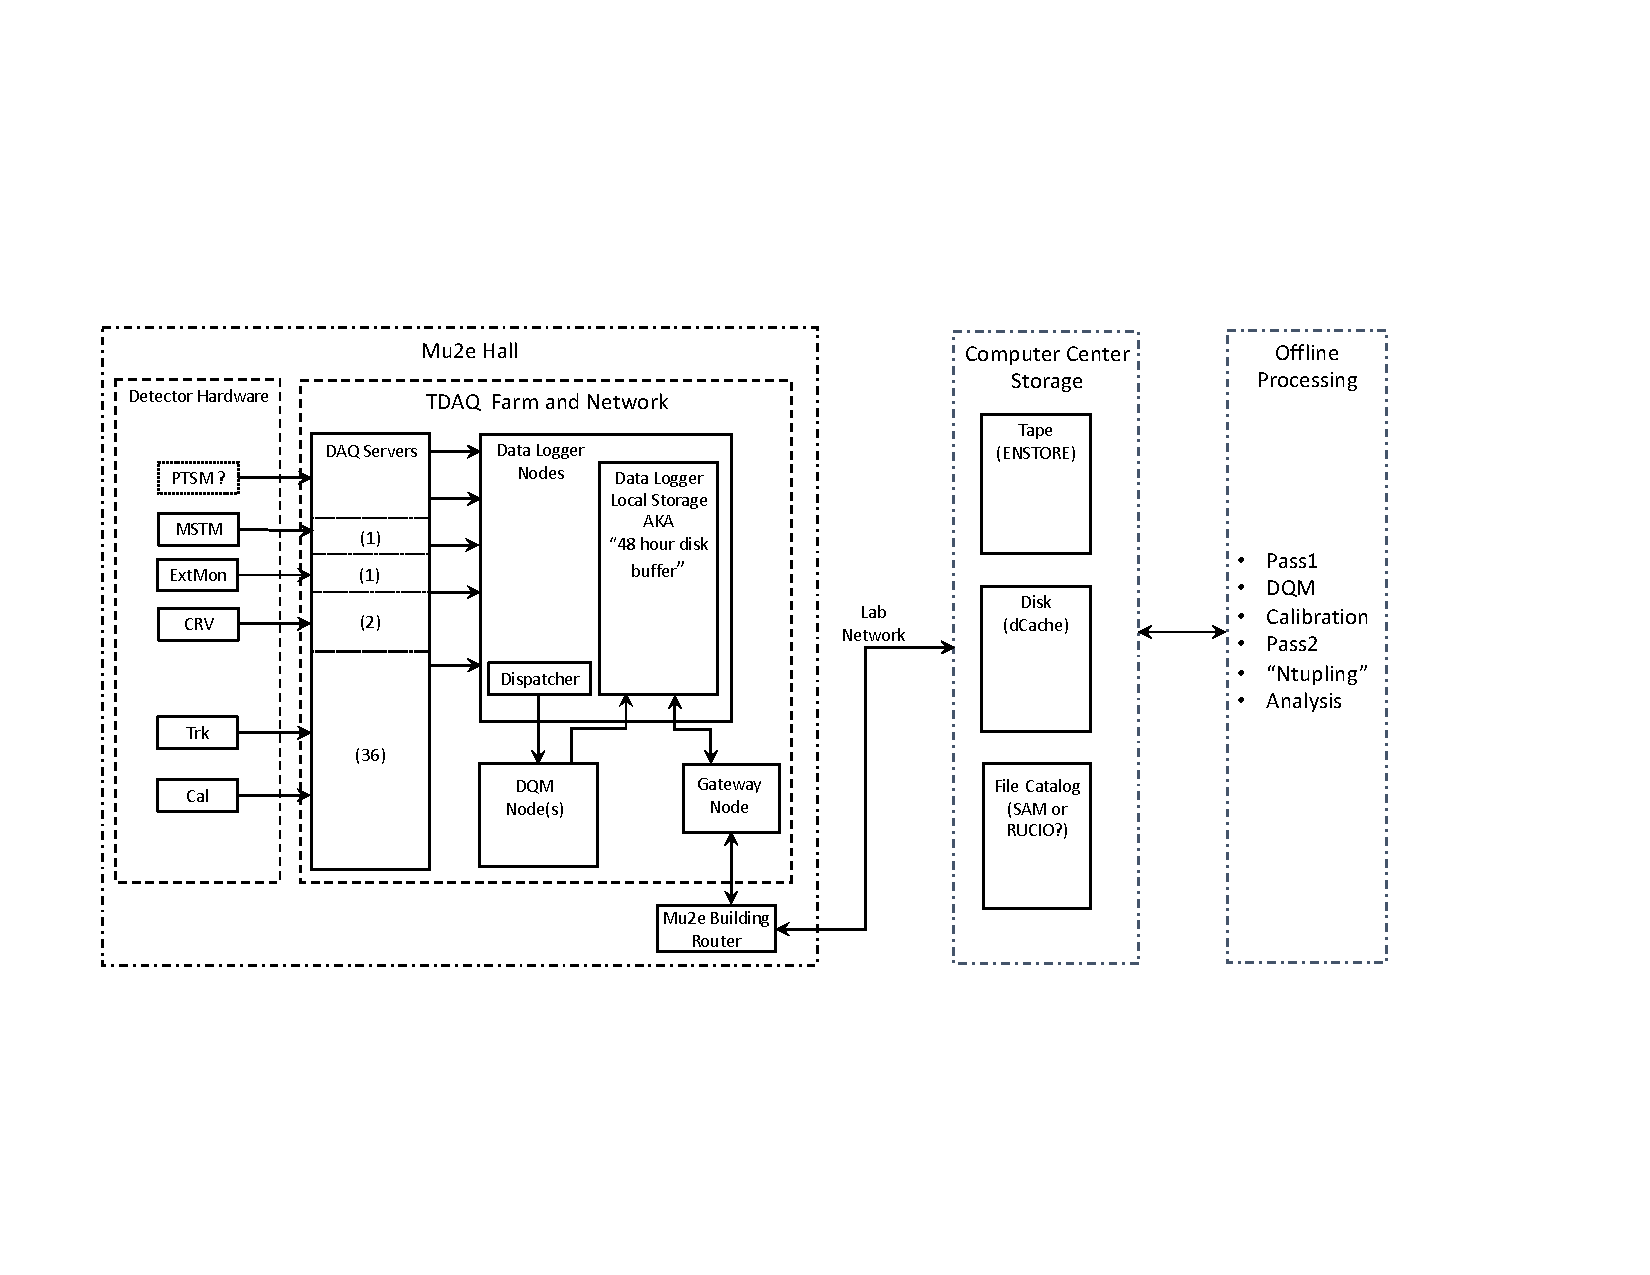
\includegraphics[width=0.9\textwidth]{figures/interface_with_TDAQ.pdf}
\caption[Block diagram of interfaces seen by the Mu2e RDM]{
  Block diagram of the interfaces seen by the Mu2e RDM.
  Not shown are \fixme{not shown}.  See the text for a discussion of these elements.}
\label{fig:blockdiagram}
\end{figure}

Data flows from the detectors, through the DAQ system into the TDAQ computer farm.
The five approved detectors are the Tracker (Trk), Calorimeter (Cal), the Cosmic Ray Veto system (CRV),
the Muon Stopping Target Monitor (MSTM) and the downstream Extintion Monitor (ExtMon).
A sixth detector has been proposed, the Production Target Scanning Monitor (PTSM),
which is drawn with a dotted box;
moreover it's primary use is to send rapid feedback to the accelerator control room
and it's not clear what, if any, data it will send through the TDAQ system.
In any event the data volume from that PTSM will be small enough that it will not be
a driver for the RDM.

A cartoon picture of the TDAQ computer farm is that it has 40 DAQ Server nodes
that talk to the detectors, build events and run trigger algorithms on those events.
The design is a deadtimeless streaming DAQ system that has no hardware trigger;
it reads every event from the detector hardware and sends all events to software filters
that run on the DAQ server nodes;
the software makes the trigger decision.
The present design is 20 software filter processes on each of the 40 DAQ server nodes, 800 total.
Events that pass the trigger are forwarded to a Data Logger node that will write the events
to files in the ``Data Logger Local Storage'', a RAID 0 disk array on the bus of the Data Logger node.
Appendix~\ref{app:DataLoggerLocalStorage} has the specs for and a discussion about this disk array.
In earlier DPC related talks and documents this was refered to as the ``48 hour disk buffer''.
In addition to the triggered events, a variety of prescaled, untriggered events will pass the
trigger and be handled the same as events that passed the trigger.
Finally, there will be special data streams for calibrations.

The base design is to have a single data logger node that receives the data from all DAQ server nodes
and writes it to files in the Data Logger Local Storage.
The data logger node will write several files, each containing events selected by a different algorithm.
Details can be found in Chapter~\ref{ch:DataStreamsAndFileStreams}.
There is an entry in the Risk Registry for the case that a technical limitation requires that
there be more than one data logger node, each of which sees only a subset
of the events; see Appendix~\ref{app:Risk:SplitFiles}.

The Data Logger nodes will also have a process called a ``Dispatcher''
that requests events from the {\code art::DataLogger} process
and forwards them to clients.
The Dispatcher is designed to exert no back pressure on the DataLogger process
and, therefore, will normally see only a subset of the events.
Two of the clients foreseen for the Dispatcher are an Event Display and
a Data Quality Monitoring (DQM) system,
which will produce histograms, timelines etc that can be viewed in real time.
Periodically the DQM system will write it's histograms, log files etc to
files in the data logger local storage.  One of the jobs of the RDM will be
to move these files to long term storage.

All of the computing resources in the TDAQ farm are on a private subnet
and cannot been seen from the lab network.  Access in and out
of the private subnet will be via a gateway node that is connected to
both the private subnet and the lab network.
Purchasing the gateway node is the responsibility of the TDAQ group.

When the Mu2e Hall was built and provisioned, CCD personnel installed a dual router
and connected it to the lab optical fiber network.
RDM will move data from the Mu2e Hall
to the computer center using this router and the lab optical fibre network.
The router is standard item that CCD uses in many places around the lab; it stocks spares.
CCD is responsible for the maintenance of both the router and the network.
See Appendix~\ref{app:RouterAndNetwork} for additional details of the arrangement with with CCD,
including costs that must be paid by Mu2e to CCD for this service.


For the foreseeable future Mu2e expects that the disk and tape services provided
by SCD will be dCache and ENSTORE.
At this writing Mu2e is using SAM as the file catalog system for files produced
by simulations, tests stands and Vertical Slice Tests (VST).
SCD plans to phase out SAM and replace it with a more modern system, RUCIO \fixme{reference};
RUCIO is already in use by CMS and by DUNE for proto-DUNE Single Phase data.
It is likely that SAM will be phased out during the lifetime of Mu2e.
One of the questions to ask in the design of the RDM is
when to make the transition to RUCIO.

\section{On-Spill, Off-Spill and Near-Spill}

This section defines the concepts of on-spill, off-spill and near-spill running.

It is expected that, for most of it's running time,
Mu2e will share parts of the Fermilab accelerator complex with a neutrino experiment,
first, with NOvA and, later, with DUNE.
To keep this document easier to read it will discuss sharing with NOvA but sharing with DUNE is implied.
The change from NOvA to DUNE may change many details
but will not materially change the requirements of the RDM.

Sharing with NOvA drives the repeating cycle of Mu2e operations, a Main Injector (MI) cycle of
21 Booster (BO) cycles;
the duration of one Booster cycle is 1/15~s,
making the duration of one MI cycle 1.4~s.
Figure~\ref{fig:beamMacroStructure} shows a cartoon of the MI cycle.
From the Mu2e point of view, the cycle starts with a series of 8 slow spills
from the Delivery Ring (DR) to the Mu2e production target;
within each spill, proton pulses arrive at Mu2e every 1695~ns;
the duration of a spill is about 43.1~ms, or about 25,500 pulses.
There is a gap of about 5~ms between spills.
The eigth spill is followed by a period of about 1020~ms,
during which no proton pulses arrive at Mu2e;
during this time, beam is delivered to NOvA
and beam is prepared for the next 8 spills to Mu2e.
Then the cycle repeats.

\begin{figure}[tbp]
\centering
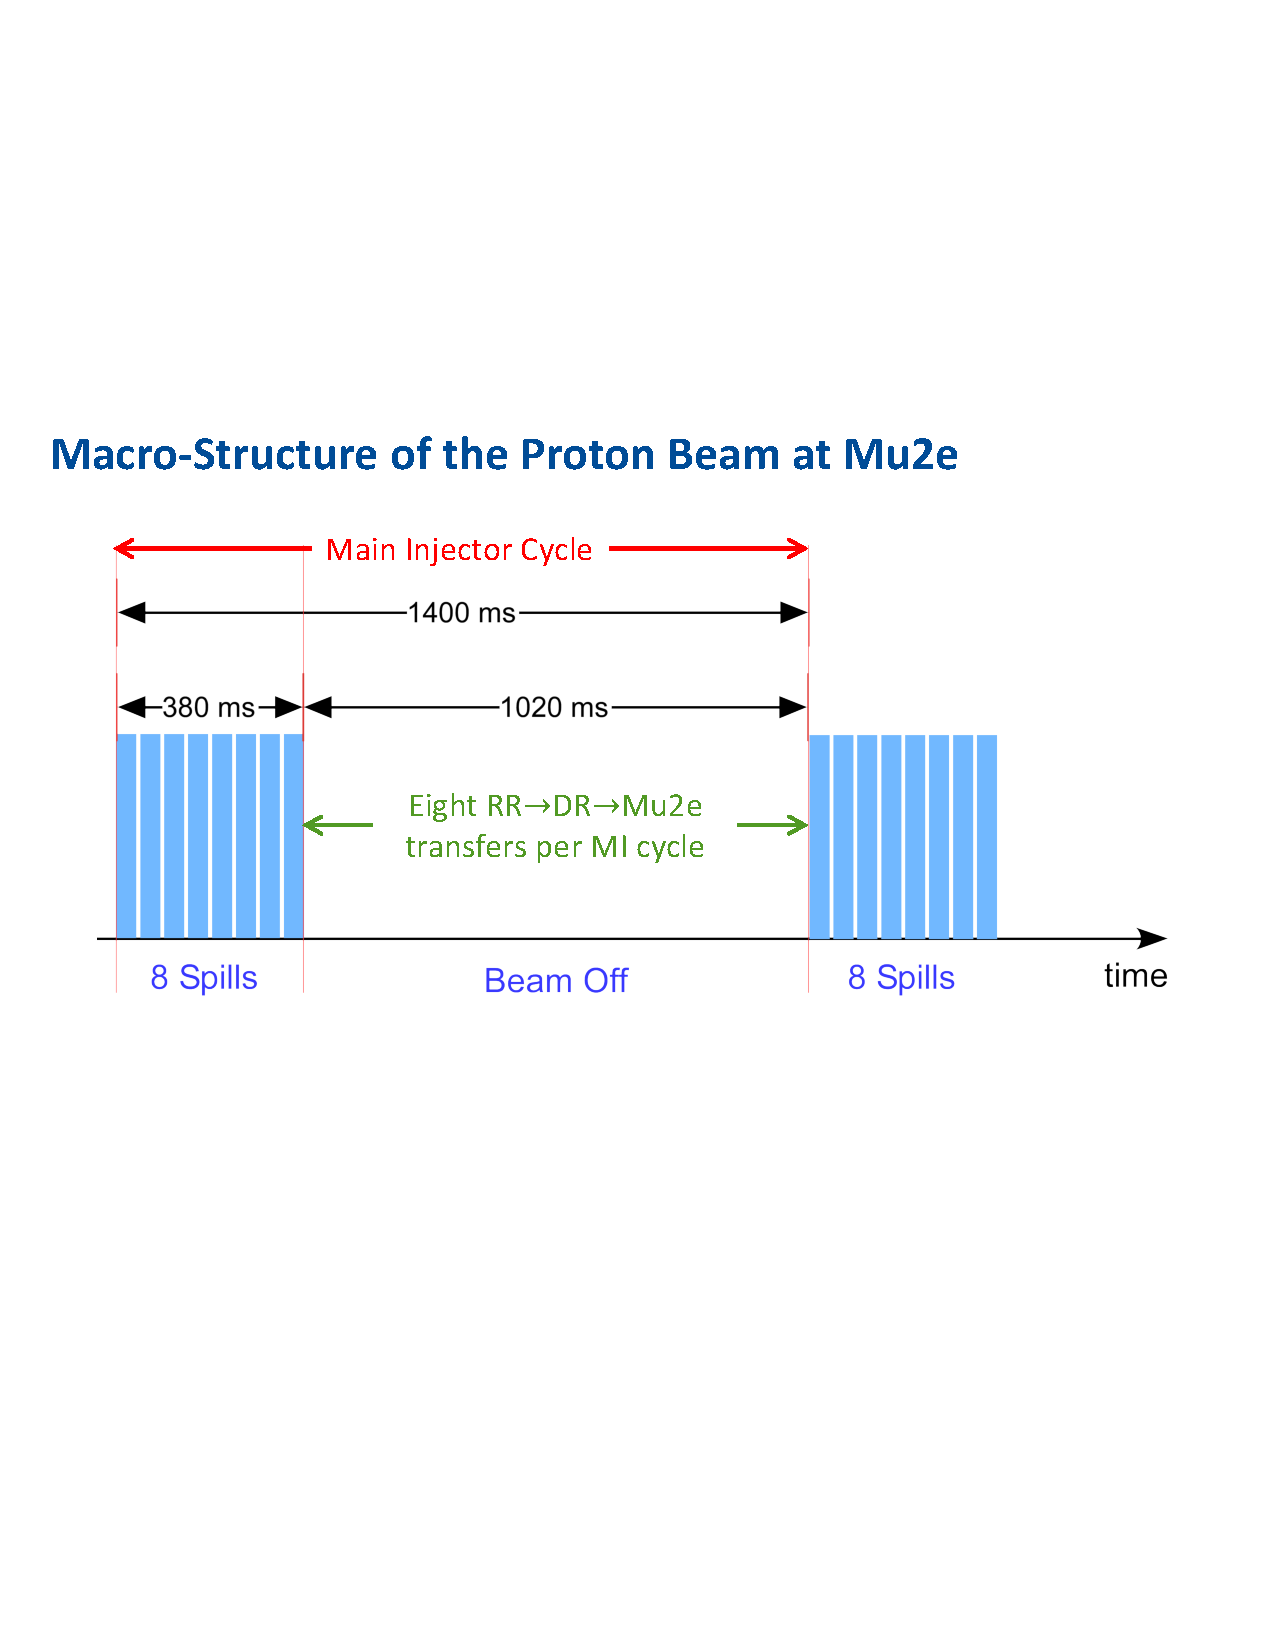
\includegraphics[width=0.9\textwidth]{figures/ProtonBeamLongitudinalStructure2019-01-10_page6.pdf}
\caption[MacroStructure of the Proton Beam at Mu2e]{
  MacroStructure of the proton beam at Mu2e, taken from page~6 of
  the file ``Proton Beam Longitudinal Structure (.pdf)'' from
  Reference~\protect{\cite{beamTiming}}.  The figure is described in the text.}
\label{fig:beamMacroStructure}
\end{figure}

During the spills, Mu2e is running in the on-spill configuration.
During the 1020~ms no-beam period, Mu2e is running in the off-spill configuration.
These two configurations are discussed below.
It has not yet been decided if the 5~ms periods between spills will
be in the on-spill or off-spill configuration
but that does not materially affect the design of the RDM.
Table~\ref{tab:timescales} summarizes the time scales within one MI cycle.
\begin{table}
\begin{center}
\caption[Numerology of the Mu2e MI Cycle]{Numerology of the Mu2e MI Cycle.}
\label{tab:timescales}
\begin{tabular}{ll}\hline
   1/15~s & Period of one Booster cycle \\
   21     & Booster cycles within the MI cycle \\
   1.4~s  & Period of one MI cycle \\
   43.1~ms & Duration of one spill \\
   8       & Number of spills per MI cycle \\
    5~ms   & Duration of the period between two spills \\
   1020~ms & Duration of the off-spill period within one MI cycle \\
   1695~ns & Period of the Delivery Ring and the duration of one on-spill event\\
   100~$\mu$s & Duration of one off-spill event \\
   24.6\%     & Duty factor (total spill time divided by MI cycle duration)\\
   \hline
  \end{tabular}
\end{center}
\end{table}


In the on-spill configuration, one event will have  a duration of 1695~ns
and it records the information associated with one proton pulse.
The trigger will be configured to select interesting events associated with the proton pulse
and to pre-scale non-triggering events in order to study the performance of the trigger.
In the off-spill configuration, one event will have a duration of 100~$\mu$s.
During the off-spill period, Mu2e will trigger on cosmic rays that
pass through the tracker and/or the calorimeter; it will also collect
pedestal data from some of the subsystems; some calibration procedures
may also take place during the off-spill period.

Mu2e expects that the accelerator super-cycle will consist of a
sequence of many of the above MI cycles,
with an occaisional other cycle mixed in.
For example, when MTEST is active, there is usually beam delivered to MTEST about once per minute.
When this occurs, Mu2e will have an extended period of off-spill running.

There will also be periods in which the accelerator complex is not delivering
beam to Mu2e for an extended time, minutes, hours, days or weeks.
In some of these periods Mu2e will shutdown to perform maintenance or repairs;
in others Mu2e will execute calibration runs;
and in others Mu2e will collect data in off-spill mode for an extended period of time.

The Mu2e TDAQ team reserved space in their configuration packet to define
a third operational mode, that they have named near-spill.
This is to allow for the possibility that some subsystems may want to
configure themselves differently during the transition from on-spill to off-spill.
At this time there are no definite plans to use this mode but it is available if needed.

The design of the Mu2e TDAQ system is that trigger processing lags the events
during the on-spill period and catches up during the off-spill period.  There is
buffering at various places in the TDAQ system to support this.

It's possible that the MI cycle might be changed to 22 BO cycles, which
will extend the duration of the off-spill period.
Also, Mu2e plans to start operations with a slightly different configuration:
4 spills instead of 8, with each spill of a longer duration than 43.1~ms.
Neither of these materially changes the requirements for the RDM and
will not be discussed further.

There will be times when Mu2e is taking data but NOvA is not.
In such times, the base plan is that Mu2e will continue to take data using the same MI cycle of 21 BO cycles.
There are several technical reasons that prevent Mu2e from reducing the off-spill period
in order to increase the duty factor.\footnote{
There are radiation safety limits on the average beam power;
the production target will have a reduced lifetime at higher average beam power;
the TDAQ system cannot accomodate a signficiantly higher event rate because it
uses the off-spill period to catch up on buffered events.
}

\section{Event WindowTags, EventIDs, Runs and Subruns}
\label{sec:TagsIDsRunsSubRuns}

Within the TDAQ system, events are identified by a 48 bit counter refered
to as the Event Window Tag (EWT);
this counter will be monotonically increasing and unique over the full Mu2e run.
The EWT is distributed by the Clock Fan Out (CFO) system to all elements of the
detector readout electronics;
it is the basis for event building.
For each Event Window the CFO also distributes a few bits to indicate the
EventMode; these bits tell the system whether it is in on-spill mode, off-spill mode
or in some other mode.

\fixme{How many bits for EventMode.  Add a reference.}

\fixme{Are there calibration modes?  For example pulsers to the calo or freon runs?}

Mu2e has chosen the \art event processing framework as it's software framework.
The software filter processes that run in the trigger farm will each be a separate \art process.
\art will also be used for offline data processing.
In \art, events are uniquely identified by a 3 part identifier called an
{\code art::EventID}; the parts are named run number, subrun number
and event number.

The TDAQ system will translate each EWT to an {\code art::EventID}
before events are presented to the \art based software filter processes.
The EWT will be recorded as part of the data payload for each event.

\fixme{ So far as I know the mechanics of mapping EWT to EventID
  is only captured in an email thread.
  Is there a real reference?
  If not, who will write it up in a referenceable way?
}

The meaning of run and subrun are defined by Mu2e.
All that \art requires is that a subrun contain zero or more
events and that a run contain zero or more subruns.

The current plan is that runs will typically have a duration of a few hours
while subruns will contain an integer number of MI cycles and
have a duration somewhere between 14 seconds and a few minutes.
This means that each subrun will contain both on-spill and
off-spill events.   The transition between subruns will
happen during the off-spill period so that each on-spill
period is contained within one subrun.

These durations are informed by the following.
Mu2e has designed a conditions management system
in which intervals of validity (IOV) are a specified as a range of subruns;
such a range may, but need not, span runs.
Therefore subruns must be short enough to follow the most
rapidly changing conditions.  As this writing it seems
likely that the upper limit for the duration of a subrun will
be set by data handling and downstream data processing considerations;
that is, files should not be too big or too small
and the follow-on data processing jobs should be able to process one subrun
in, at most, a few hours.
The Mu2e TDAQ has been designed so that subrun transitions will be deadtimeless
but that data taking will pause for a few minutes at run transitions.
The design is that the TDAQ system will do some house keeping
on run boundaries, including resetting some hardware, reloading
some firmware and restarting some processes.
These are prophylactic steps to ensure a robust TDAQ system.
Therefore a run should be long enough that the deadtime
caused by the run transition is a small fraction of the total run time
but short enough that the resets occur frequently enough
to keep the system robust.

Of course anomalies that occur during data taking will cause some runs
and subruns to be cut short.

\art has a feature that allows users to define the maximum
number of events in one file or a maximum file size.
When this feature is enabled,
and when \art detects that a limit has been reached,
it closes the output file and opens a new one.
\art provides several options to ensure distinct names for these files.
Some experiments use these features to split the events from one
subrun over many files,
keeping each file small enough for convenient data handling and data processing.
Mu2e has decided not to do this.
Mu2e will choose the duration of a subrun to ensure that this is not needed.
The language is that Mu2e will produce ``atomic subruns''; there are some
subtlties to this that are discussed in Appendix~\ref{sec:AtomicSubruns}.


\chapter{Data Streams and File Streams}
\label{ch:DataStreamsAndFileStreams}

This chapter defines the ideas of ``data streams'' and ``file streams''.
It enumerates the data streams that are anticipated at this time
and it presents a strawman for how these may be grouped into files.

\fixme{Should I use the word ``dataset'' instead of ``file stream''?
  I am using a distinct word for now since I want to reserve the word
  of dataset for something that is defined using SAM.  Are these
  two ideas identical?
}

A ``data stream'' is a series of events selected by some algorithm;
one attribute of events in a data stream is they all require the same downstream processing.
For example the on-spill and off-spill events are distinct data streams.
The on-spill events will have many trigger lines; one might consider each trigger
line it's own data stream or one might define groups of trigger lines as a data stream.
Another example: the off-spill events will include some events that triggered based on
the tracker or calorimter and they will also include events that did not trigger but
which are retained to collect a sample to study pedestals in the CRV system.
These are distinct data streams.

A ``file stream'' is a series of files that contain events from one or more data streams.
For example we might decide to bundle all of the on-spill data streams into a single
file stream or we might decide to put some of the on-spill data streams into one file
stream and another set of on-spill data streams into a different file stream.
For example all of the files containing off-spill events might be one file stream;
or maybe we will decide to split the off-spill events in to
the two off-spill data streams into two file streams.

The key point is that data streams are a fundamental idea,
while file streams are choice about how to group data streams for convenience of data handling and downstream processing.

\fixme{We need to address if a given event may be in more than one data stream.
       And we need to address if a given data stream may be in more than one file stream.
}

% Example
% Keep sections under development
\IfStrEq{\ISDRAFT}{YES}{

\chapter{A Chapter under development}
\label{ch:under_development}

This is a chapter still under development.
It is kept here to illustrate the use of the  ISDRAFT macro.

} % end `ISDRAFT = YES'

\chapter{Requirements}

This chapter lists requirements for the RDM system.
The requirements are dervived from the above firehose of information.

\begin{enumerate}
  \item Move data in a timely fashion
  \item prioritize recovery from down time.
\end{enumerate}

\chapter{Questions}

A list of questions that should be addressed in the design of the RDM:

\begin{enumerate}
\item Start by sticking with SAM and move to RUCIO later?  Or move to RUCIO now?
  How does this decision interact with requirements for ongoing simulation, VST
  and test stand work?
\item Work with TDAQ to understand the constraints that drive the choices of how to
  map data streams to file streams.
  \begin{enumerate}
    \item a separate filestream for the intensity stream.
    \item split on-spill and off-spill to separate file streams
    \item split off-spill into triggered and pedestal.
  \end{enumerate}
\item In the event of multiple data loggers, when do the files from a single subrun get joined to atomic.
\end{enumerate}


\appendix

\chapter{Network Between Mu2e Building Router and Computer Center}
\label{app:RouterAndNetwork}.

The Mu2e building router is owned by CCD.
\begin{itemize}
\item specs; dual; auto fail over; channels; free to increase \#channels
\item Router is owned and maintained by CCD; stock item so they can replace quickly.
\item We pay yearly maintenance: \fixme{Amount in FY21 and inflation estimate}
\item We pay for replacement; we pay CCD and they do the work. \fixme{when is next replacement due; replacement cycle}
\item \fixme{make sure this is in MOU} Coverage.
\item \fixme{not sure who paid for the existing one.}
\end{itemize}


The lab network.
\begin{itemize}
\item Install and maintained by CCD.
\item Normal maintenance and repair is budgeted for in their ops budget
\item If there were an emergency repair that exceeded their budget they would come to us. \fixme{make sure this is covered in MOU}
\end{itemize}

\chapter{Data Logger Local Storage}
\label{app:DataLoggerLocalStorage}

\fixme{ Specs etc on the Data Logger Local Storage go here}.

\chapter{Things to Know About \art}

This chapter describes details of \art that should be considered when
designing the RDM.  This includes details that are important for the RDM
proper and details that are important when shaping data for downstream
processing.

\section{Atomic Subruns}
\label{sec:AtomicSubruns}

A subrun is said to be ``atomic'' if all of the events in that subrun are found in a single \art file.
If subruns are atomic, some bookkeeping operations are simplified and Mu2e plans to exploit this;
therefore the TDAQ and RDM should aim to create atomic subruns as early as possible in the workflow.

Why ``as early as possible'' and not ``must''? 

The base design of the TDAQ is to have one {\code artdaq::DataLogger} process that will
see all events and write them to disk; it may write several output files.
However it is possible that a single {\code artdaq::DataLogger} will not have the
resources to handle the load.  Should that happen the solution is to have two
{\code artdaq::DataLogger} processes, each of which sees about half of the events.
In this case all of the output files will be duplicated,
one for each {\code artdaq::DataLogger}.
In this case subruns are not atomic;
the RDM and DPC will need to work together to decide where in the workflow these two files
are joined to create atomic subruns.

There is an additional subtlety.
Section~\ref{sec:TagsIDsRunsSubRuns} described that Mu2e subruns will cover many MI cycles
and, therefore, will include both on-spill and off-spill events.
One option for the TDAQ, the option that is preferred by DPC,
is that TDAQ will write on-spill and off-spill events to separate files.
The Mu2e DPC anticipates only workflows in which these two files are treated separately;
another way of saying it is that there will be no jobs that read events from both of these files.
Therefore we can say that within each of these two file streams the design is for subruns to be atomic.
This is the usual meaning of ``atomic subrun'' throughout this document.

\subsection{Sparse Skims}

This section assumes that the reader is familiar with the \art concepts
of data products that are held by the {\code art::Run} object
and data products that are held by the {\code art::SubRun} object.
It also assumes that the reader is familiar with the \art concepts
of {\code art::Run} and {\code art::SubRun} fragments
and with the concept of aggregation for these fragments.
For information about these concepts see~\cite{RunAndSubRunProducts}
and~\cite{ProductAggregation}.


By default \art assumes that subruns are not atomic
but you can tell \art that subruns will be atomic by adding this fcl
parameter to the parameter set of the RootInput module

\cmd{ compactEventRanges : true}

When \art sees a beginRun transition, it reads all run data products from the input file.
When \art is configured for atomic subruns, it drops these data products
from memory at the matching endRun transition.
Similarly, when \art has beginSubRun transition, it reads all subrun data products from the input file.
When \art is configured for atomic subruns, it drops these data products
from memory at the matching endSubRun transition.
When \art is not configured for atomic subruns it does not drop these data products from
memory at the matching endSubRun transition; the reason is that 

On the otherhand, when art is configured for non-atomic subruns

When \art is configured for non atomic subruns there is an extra memory cost;
for sparse skims this can dominate the memory usage of the process.
While this added memory cost is small early in the production, chain when
only a few subruns are seen by any given process, it's important to be
aware of this constraint when shaping the data for downstream processing.

To understand how the memory cost arises,
it is necessary to understand the structure of an art file.
Suppose that you have an art file with run:subrun ( 1:1, 1:2, 2:1, 2:2).
When you read the art file you will see the sequence of records shown
in table~\ref{tab:atomicsubruns}.

\begin{table}
\begin{center}
\caption[Example For Discussion of Atomic Subruns]{Example for the Discussion of Atomic Subruns}
\label{tab:atomicsubruns}
\begin{tabular}{l}\hline
  begin run record for run 1 \\
  begin subrun record for subrun 1:1 \\
  records for the events of subrun 1:1 \\
  end subrun record for subrun 1:1 \\
   begin subrun record for subrun 1:2 \\
   records for the events of subrun 1:2 \\
   end subrun record for subrun 1:2 \\
   end run record for run 1. \\ \hline
   begin run record for run 2. \\
   begin subrun record for subrun 2:1 \\
   records for the events of subrun 2:1 \\
   end subrun record for subrun 2:1 \\
   begin subrun record for subrun 2:2 \\
   records for the events of subrun 2:2 \\
   end subrun record for subrun 2:2 \\
   end run record for run 2. \\
   \hline
  \end{tabular}
\end{center}
\end{table}

Now suppose that your job reads the run and subrun scope data products at begin run/subrun time.
If \art is configured for atomic subruns, after processing the module and service
{\code endSubRun} calls, it will delete the subrun data products from memory. It can safely do this
because it knows that it will never see another event from that subrun.
Similar for the run scope data products.

On the other hand, if \art has been configured for non-atomic subruns, it will retain all subrun
and run data products in memory until the end of the job.
For a job that sees a small number of subruns this is usually not an important memory cost; but
for sparse skims it can be dominant.


There is a second consideration about atomic subruns:
for sparse skims there is signficant memory savings if subruns are atomic.
While the RDM will not see sparse skims, the people developing it should know the big picture.


\section{Order of Events}

\chapter{Risk Registry}
\label{app:RisKRegistry}

\section{Split Files from DAQ}
\label{app:Risk:SplitFiles}

The base design is to have a single data logger node that receives data from all DAQ server nodes.
This design cannot be tested at scale until all of the hardware has been purchased;
even then, the tests will be based on simulated events, not actual data.
There is a risk that there will be a bandwidth limit that makes this impossible.
Should this occur, there backup plan is to have two or more Data Logger nodes
that each see a fraction of the events;
perhaps half of the DAQ Servers talk to one Data Logger node and the other half talk to another node.
The result will be that events from the same file stream from the same subrun end up split across multiple files.
This breaks the requirement that subruns be atomic.

Should this occur the RDM will need to modify the bookkeeping system to allow non-atomic subruns early
in the workflow and modify the workflow to restore atomic subruns as soon as possible.

Another alternative is to tighten the trigger algorithms to accept fewer events;
this risks loosing events that we really do want to keep and is the last alternative.

\clearpage
\phantomsection
\addcontentsline{toc}{chapter}{Bibliography}
\printbibliography


%\cleardoublepage
%\printindex
